\begin{figure*}[ht]
\begin{tabular}{@{}c@{\hspace{0.005in}}c@{\hspace{0.005in}}c@{}}
	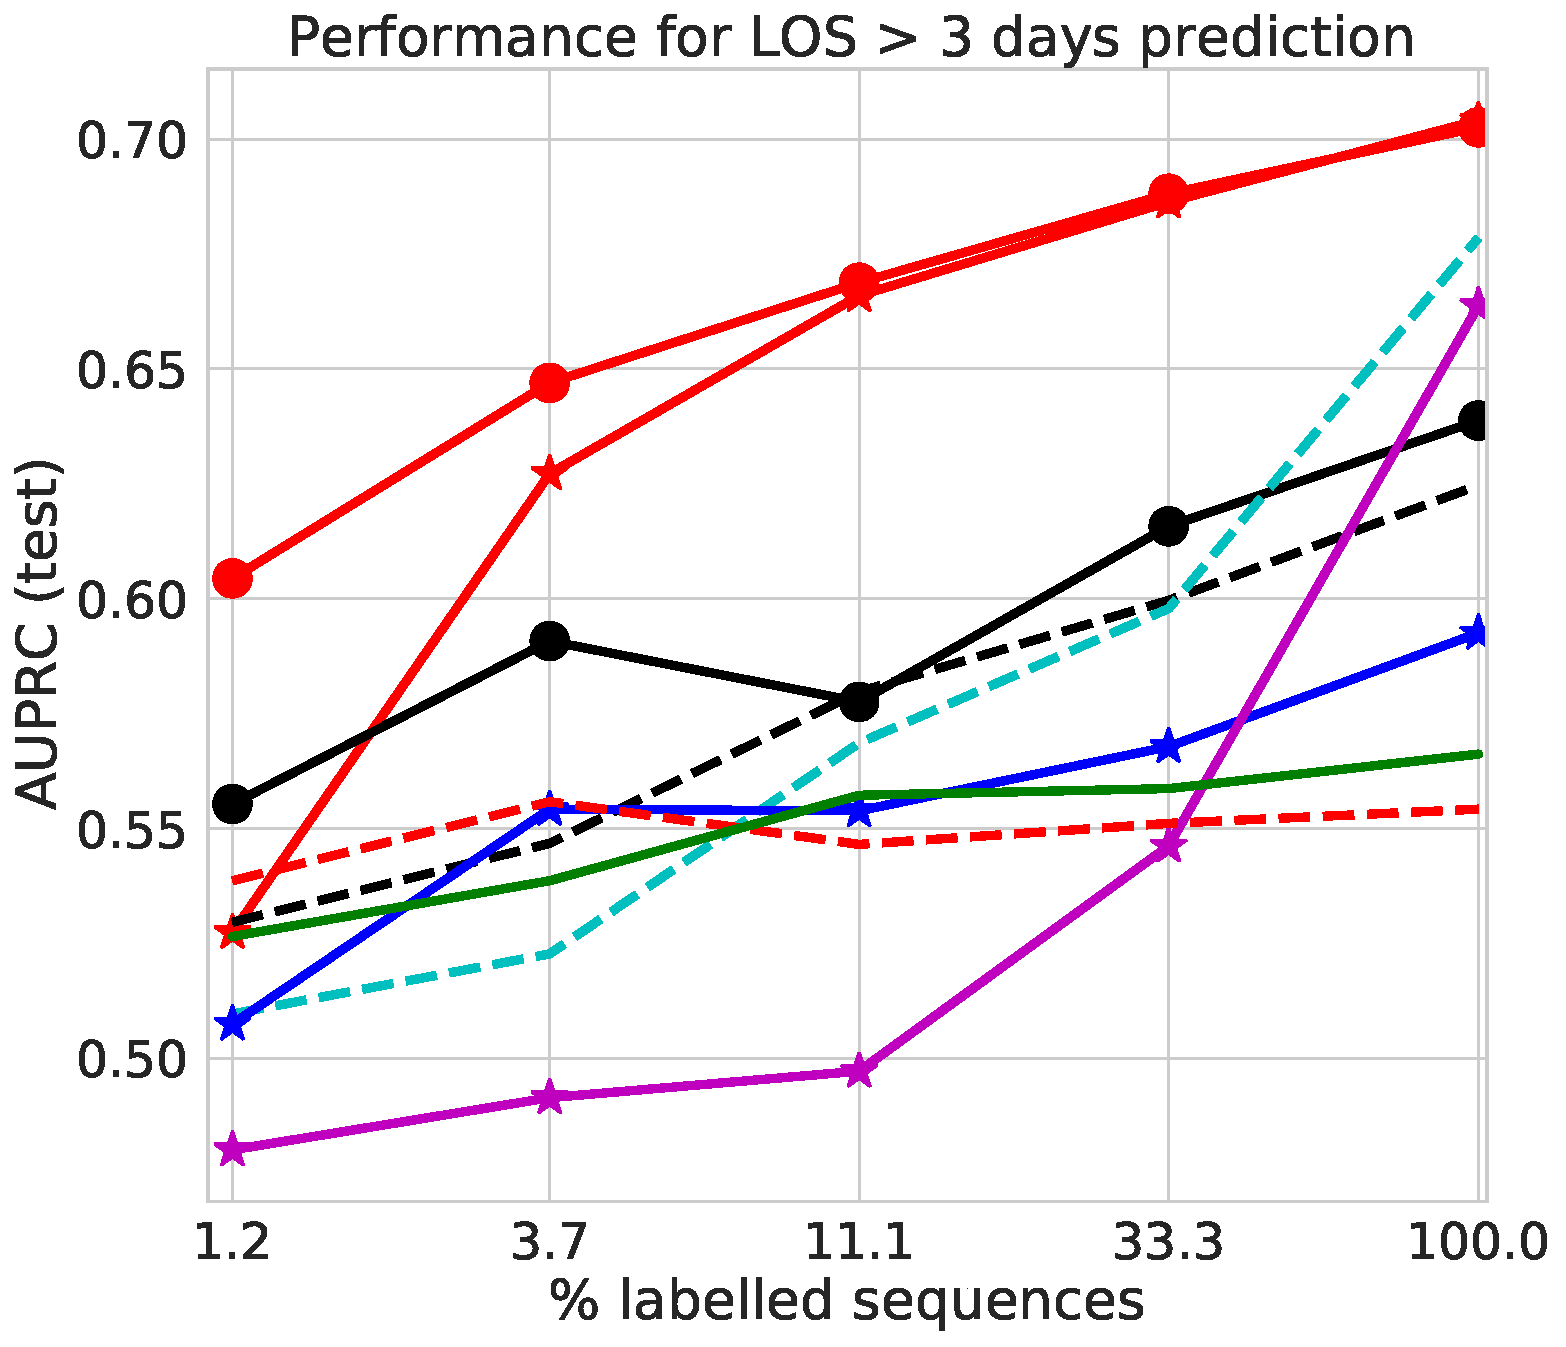
\includegraphics[width=0.35\textwidth]{content/chapters/semi_supervised_pchmm_missing_data/images/perf_los_geq_3_days.pdf}
	&
	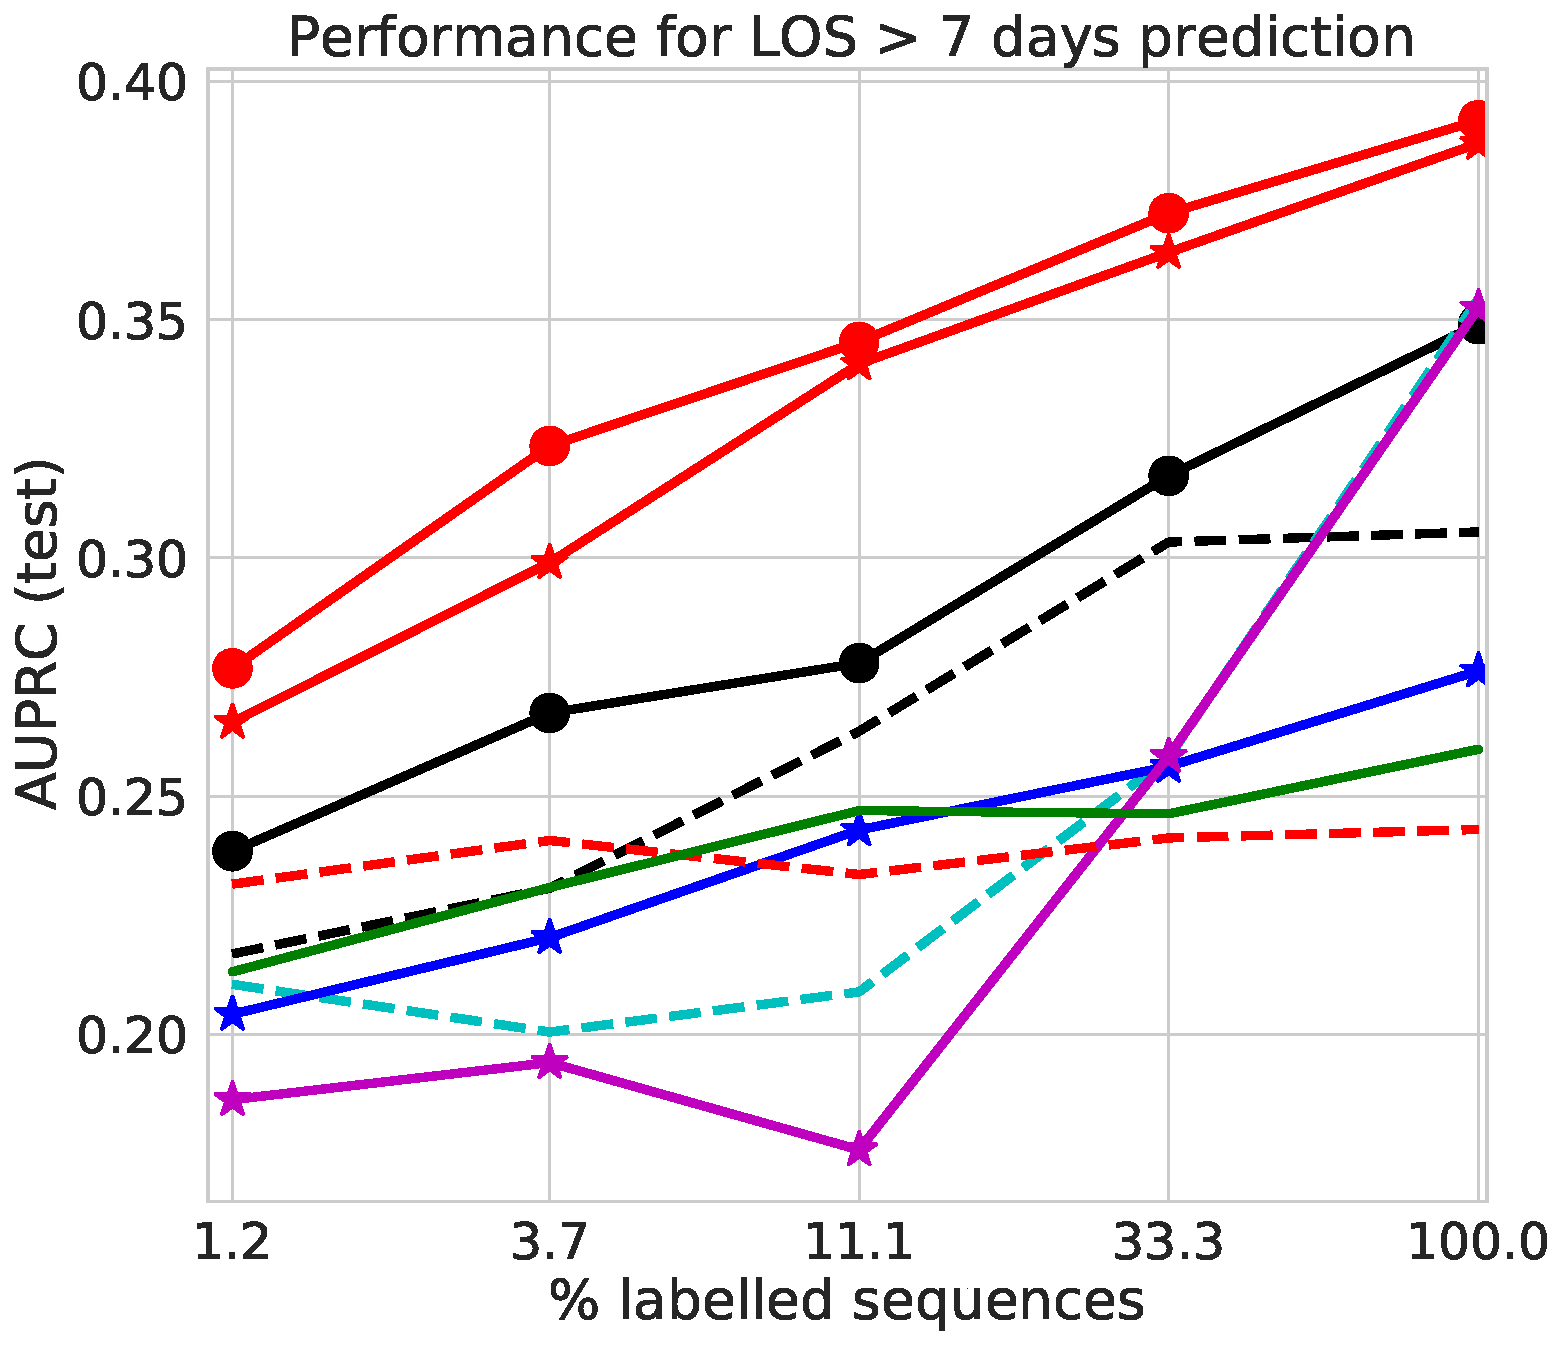
\includegraphics[width=0.35\textwidth]{content/chapters/semi_supervised_pchmm_missing_data/images/perf_los_geq_7_days.pdf}	
 	&
	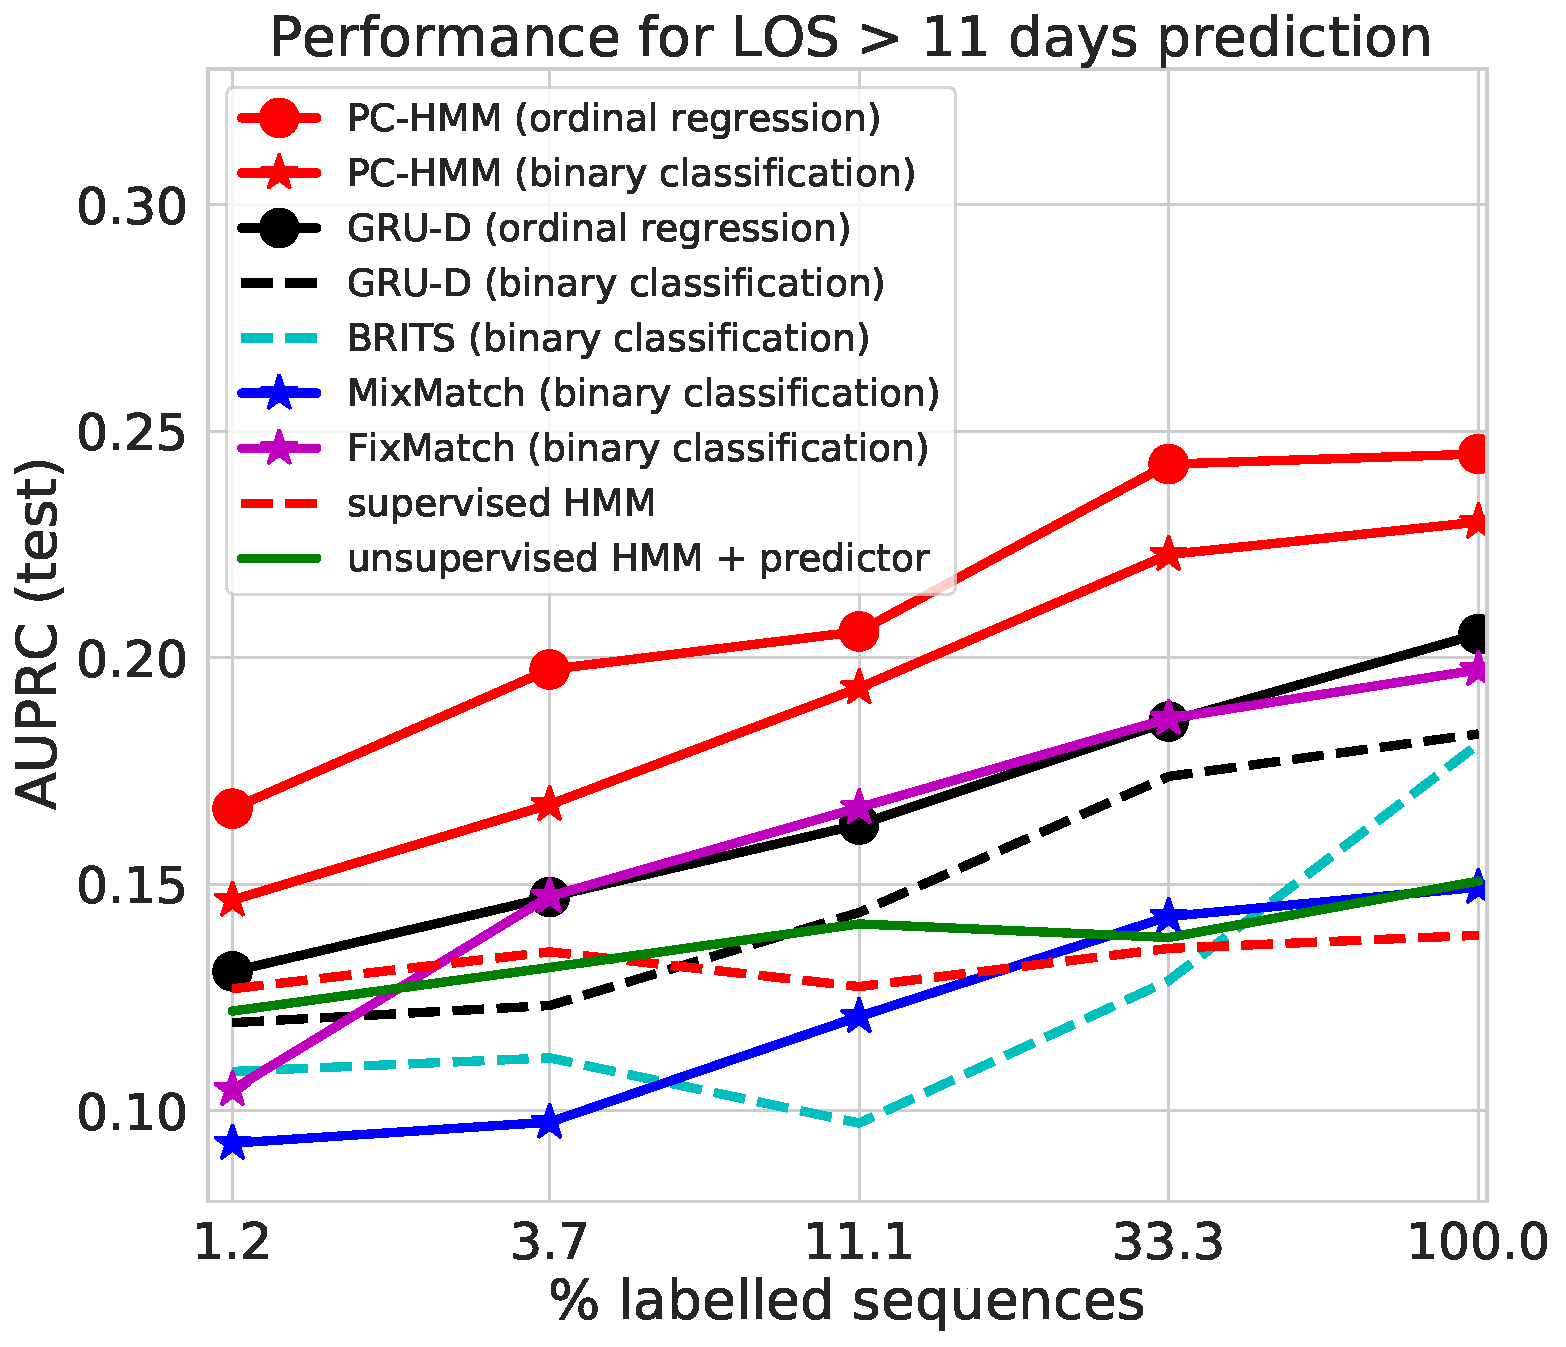
\includegraphics[width=0.35\textwidth]{content/chapters/semi_supervised_pchmm_missing_data/images/perf_los_geq_11_days.pdf}	
\end{tabular}
\caption[AUPRC versus amount of labeled data for length-of-stay prediction on MIMIC-IV at 3 ordinal labels ($>3$, $>7$, and $>11$ days)]{AUPRC (higher is better) versus amount of labeled data for length-of-stay prediction on MIMIC-IV at 3 ordinal labels ($>3$, $>7$, and $>11$ days).
SSL methods (PC-HMM, MixMatch, and FixMatch)
learn from both labeled and unlabeled data.
GRU-D \citep{cheRecurrentNeuralNetworks2018} and BRITS \citep{caoBRITSBidirectionalRecurrent2018} use the labeled set only.
Binary classification models require 3 separate models (1 for each label), whereas ordinal regression using CLMs require a single model to predict all 3 labels. }%endcaption
\label{fig:MIMIC_los_prediction_results}
\end{figure*}